% ~ 3-4 pages
\chapter{Reconstruction, Energy Calibration and
  Identification of Hadronic Tau Lepton Decays}
\label{sec:reconstruction}

% TauBuilder config:
% https://gitlab.cern.ch/atlas/athena/blob/master/Reconstruction/tauRec/python/TauRecBuilder.py
%
% AlgHolders:
% https://gitlab.cern.ch/atlas/athena/blob/master/Reconstruction/tauRec/python/TauAlgorithmsHolder.py
%
This chapter summarises the offline reconstruction procedure used at ATLAS to
reconstruct hadronic decays of tau leptons as given in \cite{atlas:taurec:run1,
  atlas:taurec:run2}. Additionally recent changes to the reconstruction
algorithms are included (packages \texttt{tauRec}, \texttt{tauRecTools} in the
software framework \textsc{Athena}).

% JetSeedBuilder:
% https://gitlab.cern.ch/atlas/athena/blob/master/Reconstruction/tauRecTools/src/JetSeedBuilder.cxx
Candidates for hadronic tau decays are seeded by jets formed by the
anti-$k_\mathrm{t}$ jet algorithm using a distance parameter of $R = 0.4$ on
three-dimensional clusters of calorimeter cells called \emph{TopoClusters}
calibrated using the local hadronic calibration (LC-scale)
\cite{local_hadronic_calib}\todo{accounts for non-compensating nature of the
  calo by classifying clusters as em or hadronic, dead material, out-of-cluster
  energy of low-pt particles that are bent from the jet}. The jet seed has to
satisfy $p_\mathrm{T} > \SI{10}{GeV}$ and is required to fall into the
acceptance range of the tracking system $|\eta| < \num{2.5}$. \todo{At this step
  tau $p_\mathrm{T}, \eta, \varphi, m$ ($m$: invariant mass) are set to the ones
  of the jet seed -- what does this mean? Read up on jet algs}

% TauVertexFinder:
% https://gitlab.cern.ch/atlas/athena/blob/master/Reconstruction/tauRecTools/src/TauVertexFinder.cxx
%
% Vertex association: Tracks matched unambiguously to jets via ghost-matching by
% adding all tracks into constituent list for the jet algorithm but setting
% their energy infinitesimally small (such that the result of the jet algorithm
% is not affected due to IR-safety) and rerunning the algorithm.
% \url{https://twiki.cern.ch/twiki/bin/view/AtlasProtected/JetGhostMatching}
%
% Tracking CP recommendations
% \url{https://twiki.cern.ch/twiki/bin/view/AtlasProtected/TrackingCPPreRecsSummer2017#Track_to_Vertex_Association}
In events with multiple primary vertices the tau production vertex has to be
identified. Reconstructed tracks associated to the calorimeter jet via
ghost-matching\footnote{Tracks matched unambiguously to calorimeter jets by
  adding the tracks with infinitesimal energy to the constituent list and
  rerunning the jet algorithm.} that lie in a cone of $\Delta R < 0.2$ with
respect to the jet axis and fulfil $p_\mathrm{T} > \SI{1}{\giga\electronvolt}$
and basic track quality criteria $N_\mathrm{Pixel} \geq 2$ (PixelHits +
PixelDeadSensors) and $N_\mathrm{Si} \geq 7$ (PixelHits + SCTHits +
PixelDeadSensors + SCTDeadSensors) are selected. The primary vertex is
then associated to be the one maximising the Jet Vertex Fraction
\begin{align*}
  \mathrm{JVF} = \frac{\sum_\text{Vtx.\ \& TJVA} p_\mathrm{T}}
                                           {\sum_\text{TJVA} p_\mathrm{T}}
\end{align*}
given by the ratio of the $p_\mathrm{T}$ sum of all selected tracks that are
also matched to the vertex\footnote{Impact parameter based association with the
  primary vertex. $|d_0| < \SI{2.5}{mm}$ with respect to beamline and
  $|(\Delta z_0) \sin\theta| < \SI{3}{mm}$. $\Delta z_0$ is the longitudinal
  distance of vertex and track} to the sum of $p_\mathrm{T}$ of all selected
tracks.

% TauAxisSetter:
% https://gitlab.cern.ch/atlas/athena/blob/master/Reconstruction/tauRecTools/src/TauAxisSetter.cxx
The LC calibrated energy of the tau is set to the energy of all
\emph{TopoClusters} within a cone of $\Delta R < 0.2$ with respect to the
barycentre\footnote{$\eta$ and $\phi$ of the four momentum vector given by the
  sum of all cluster 4-momenta.} of all clusters of the jet at LC scale
(\texttt{ptDetectorAxis}) and is the baseline for further energy calibration
\todo{This part could be in the first paragraph}. Finally the tau axis ($\eta$,
$\phi$\footnote{strictly also $p_\mathrm{T}$ as a result}) is corrected for the
position of the primary vertex (\texttt{ptIntermediateAxis}). After the axis
correction and the identification of the primary vertex, the track impact
parameters can be recalculated with respect to the primary vertex (like for
z0sinThetaTJVA).

% TauTrackFinder:
% https://gitlab.cern.ch/atlas/athena/blob/master/Reconstruction/tauRecTools/src/TauTrackFinder.cxx
%
% TauTrackClassifier:
% https://gitlab.cern.ch/atlas/athena/blob/master/Reconstruction/tauRecTools/Root/TauTrackClassifier.cxx
Reconstructed tracks in the inner detector are associated with a reconstructed
hadronic tau decay if they are within the cone of size $\Delta R < 0.4$ centred
on the tau axis (corrected for the PV).
% The tracks are classified into core, wide, and other tracks: If the tracks
% fail track selection (pt > 1GeV, IPd0Max = 1mm, IPz0Max = 1.5mm, nHitPix >= 2,
% nHitSi >= 7) they are classified as 'other'.
%
% If the tracks are within the 0.2 cone they are called 'core' tracks otherwise
% if they fall into the 0.2 - 0.4 annulus they are classified as 'wide'.
%
% Loose track selection for charged pions according to TrackingCP:
% pt > 400 MeV (This cut is already applied at track reco)
% |eta| < 2.5
% NSi >= 7
% N^sh_mod <= 1 (Number of shared models = N^sh_Pix + N^sh_SCT / 2)
% N^hole_Si <= 2
% N^hole_Pix <= 1
%
% Dirk's talk in TauCP:
% https://indico.cern.ch/event/615208/contributions/2481630/attachments/1415563/2167141/TauCP_TrackClassificationTaskforce_20170220.pdf
For each track a multi-class classification is performed categorising them in to
four track-categories: charged (TT), conversion (CT), isolation (IT) and fake
(FT). Charged or tau-tracks are charged pion tracks from the decay of the
tau-lepton, conversion tracks are long-lived secondary particles from converted
photons (e.g.\ from $\pi^0$-decays) or hadronic interactions, isolation tracks
are primary particles that are not originating from the tau-decay and includes
tracks from the underlying event, fake tracks are reconstructed tracks with a low
truth-matching probability in simulation (i.e.\ tracks reconstructed from
pile-up hits?). \todo{Does this make sense?}. This is
done using three boosted decision trees performing binary classifications of the
charged \& conversion vs.\ isolation \& fake categories and subsequently
classifying (in preliminary categories) charged vs.\ conversion and isolation
vs.\ fake. \todo{Figure with schematic of BDT setup, Input variables} The charge
of the reconstructed tau-lepton is calculated by summing the track charge of all
tracks classified as 'charged' which also defines the \todo{prongness} of the
decay. This algorithm is optimised to classify the tracks such that the tau is
reconstructed with the correct number of charged tracks (i.e.\ 1 or 3) to
improve reconstruction efficiency \todo{This is a problem for algorithms relying
  on isolation/fake tracks}. For identification purposes an additional
classification as 'modified isolation tracks' was introduced given by tracks
that are not classified as 'charged' and fulfil track selection
criteria\footnote{Transverse momentum:
  $p_\mathrm{T} > \SI{1}{\giga\electronvolt}$, Impact parameters w.r.t.\ the
  interaction point (TJVA): $d_0^\text{IP} < \SI{1}{mm}$,
  $|z_0^\text{IP}| \sin\theta < \SI{1.5}{mm}$; Track quality criteria:
  $N_\text{Pixel} \geq 2$ and $N_\text{Si} \geq 7$}. This category is used to
calculate the isolation variables SumPtTrkFrac and massTrkSys \todo{Ref to
  section where these are defined}.

\todo{NTrack requirement for analyses and rejection due to this requirement}
% Tau Tracks: tracks from the direct tau decay (pions)
%
% Conversion Tracks: tracks from conversions, hadronic interactions, 'long'
% living particles MVA Tracking input (barcode > 200k -- secondary particles)
%
% Isolation Tracks: mainly tracks from the underlying event (barcode < 10k but
% not tau tracks)
%
% Fake Tracks: not truth matched (10k < barcode < 200k) (includes pilup?)
%
% barcode < 200k -- primary particles
%
% variables: jetseed pt, track eta, z0SinThetaTJVA, rConvII, dRJetSeedAxis, d0,
% qOverP, nInnermostPixelHits, nPixelSharedHits, nSCTSharedHits, eProbabilityHT,
% nPixHits, nSiHits
% Impact params: reject conversion (d0), isolation and fake tracks (z0)
% Pixel, Si-Hits: rejection against conversions (missing hits)
% shared hits: intent is to recover merged tracks
% eProbabilityHT: Conversion tracks
% qOverP, dR: IT, FT

% TauCalibrateLC:
% https://gitlab.cern.ch/atlas/athena/blob/master/Reconstruction/tauRecTools/Root/TauCalibrateLC.cxx
%
% 5 eta bins: [0.0, 0.3, 0.8, 1.3, 1.6, 2.4]
% pile-up slopes for 1P and 3P for each eta bin
% mean pile-up for 1P and 3P
% A calibration function for 1P and 3P for each bin
%
% Offset calculated as
% offset = slope * (reco. num of PU vertices - average number of PU vertices)
% energyLC = ptDetectorAxis()
% if energyLC - offset <= 0: set offset to 0
% energyPUCorr = energyLC - offset
% calibConst = func(nProng, eta; energyPUCorr)
% if calibConst <= 0: calibConst = 1.0
% energyFinal = energyPUCorr / calibConst
%
\todo{Motivation: LC scale not optimised for tau energy measurement; e.g.
  hadronic composition of the final state, pile-up, cone size of 0.2. Reduce
  bias and improve resolution} To get the visible tau energy a further energy
calibration is applied to the tau candidates to account for pileup and the
detector response in different $\eta$ regions. First the pileup contribution
$E_\text{PU}$ to the energy at LC-scale $E_\text{LC}$ is estimated using
\todo{Does the LC-scale already account for the average pile-up? Otherwise the
  parametrisation subtracting the average number of pile-up vertices would not
  make sense! The LAr bipolar calorimeter signal should cancel the in-time
  pile-up with the out-of-time pile-up.}
\begin{align*}
  E_\text{PU} &= m\left(|\eta|\right) \times \left( N_\text{Vtx.}^\text{PU}
                - \langle N_\text{Vtx.}^\text{PU} \rangle \right) \eqcomma
\end{align*}
where $m$ is the average pile-up contribution to the energy at LC-scale (is a
function of $|\eta|$) parametrised in bins of eta separately for 1- and
multi-prong taus. Finally the energy is corrected for the detector response (in
bins of $|\eta|$ and separately for 1- and multi-prong).
\begin{align*}
  E_\text{TES} &= \frac{E_\text{LC} - E_\text{PU}}
                 {\mathcal{R}(|\eta|, E_\text{LC} - E_\text{PU})}
\end{align*}
The detector response function $\mathcal{R}$ is fitted to the mean of the
$\frac{E_\text{true}}{E_\text{LC} - E_\text{PU}}$ distributions (from a Gaussian
fit) in simulation for each bin using a function with an empirical form.

% TauShotFinder
% https://gitlab.cern.ch/atlas/athena/blob/master/Reconstruction/tauRecTools/src/TauShotFinder.cxx
Local maximum in EM1 strip layer determined by cells within 0.2 (0.4?) to the
tau axis. Cells required to have above \SI{100}{\mega\electronvolt}. Two seed
cells can't be neighbours in eta. Seed cell must be local maximum in eta (both
neighbours are required to have lower cell energy). Shot construction: Seed
cells neighbouring a seed cell in phi direction are merged (only the highest pt
neighbour is merged). A cluster is built in a 5 (eta) x 1 (phi) window around
the seed or 5 x 2 in case a neighbouring seed was merged in. The four-momentum
is set to the cell energy/eta/phi of the seed cell or in case of merged seeds to
the sum of the seed cell pt and the barycentre of energy in phi direction. The
number of photons in the shot is calculated as a function of 5 $|\eta|$ bins
($0, 0.8, 1.39, 1.51, 1.8, \infty$). If the seed energy (energy in a window of
width 3x1(2)) is smaller then a threshold no photon is counted. If it exceeds
the threshold \{430 MeV, 300 MeV, crack, 330 Mev, 350 MeV\} one photon is
counted. In case the shot energy exceeds 10 GeV the photon is counted twice.


\todo{Cite ATHENA?}

\section{Vertex Association}
\label{sec:reco_vertex_assoc}

\section{Track Selection and Classification}
\label{sec:reco_track_sel_classif}

\begin{figure}[ht]
  \centering
  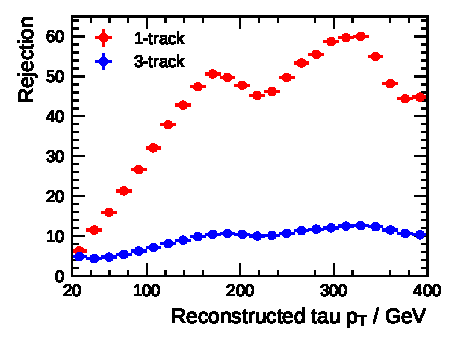
\includegraphics{./figures/bdt_perf/mva_tracking_rejection.pdf}
  \caption{Rejection due to MVA tracking \todo{Why is the rejection 'wavey'?}
    Rejection of tau candidates from dijets after baseline tau selection.}
  \label{fig:mva_tracking_rejection}
\end{figure}

\section{Energy Calibration}
\label{sec:reco_energy_calib}


% -------------------------- FIRST DRAFT ------------------------------ %
\begin{itemize}
\item Building jet seed from AntiKt4LCTopoJets ($p_\mathrm{T} > \SI{10}{GeV}$)

\item Vertex finding \& TJVA (Track Selection $\Delta R < 0.2$ \& PixHits /
  SiHits requirement, Jet Vertex Fraction)

\item Energy \& axis calculation (clusters within $\Delta R < 0.2$ w.r.t.
  barycentre associated with tau [ptDetectorAxis], correct axis for vertex
  position [ptIntermediateAxis])

\item Track selection \& track classification (MVA tracking TT/CT/IT/FT, sets
  charge/prongness, modifiedIsolationTracks, Multijet rejection from
  \texttt{nTrack} requirement)

\item Energy Calibration: LC \textrightarrow TES (Separately for 1-prong and
  multi-prong: subtract PU energy using $N_\mathrm{PV}$ / $\mu$, apply
  calibration factor depending on $|\eta|$ \& $E_\mathrm{LC} - E_\mathrm{PU}$

\item Tau-ID (Could be moved to next chapter?)

\item Substructure Reconstruction (?)
\end{itemize}

% -------------------------- ??? -------------------------------- %

\begin{itemize}
\item Jet seed
\item TJVA
\item MVA tracking (Rejection due to track requirement)
\item Identification (jet veto, electron veto, muon veto)
\item Tau Particle Flow \& Decay Mode Classification
\end{itemize}

\cite{atlas:taurec:run1}
\cite{atlas:taurec:run2}
\cite{atlas:taurec:decaymodes}

%%% Local Variables:
%%% mode: latex
%%% TeX-master: "mythesis"
%%% End:
